\RequirePackage{docswitch}
% \flag is set by the user, through the makefile:
%    make note
%    make apj
% etc.
\setjournal{\flag}

\documentclass[\docopts]{\docclass}

% You could also define the document class directly
%\documentclass[]{emulateapj}

% Custom commands from LSST DESC, see texmf/styles/lsstdesc_macros.sty
\usepackage{lsstdesc_macros}
\usepackage{rotating}
\usepackage{graphicx}
\usepackage{diagbox}
\usepackage{multirow}

%\usepackage{pdflscape}
\graphicspath{{./}{./figures/}}
\bibliographystyle{apj}

% Add your own macros here:
\newcommand{\snrb}{\mbox{$SNR^b$}}
\newcommand{\snrbmin}{\mbox{$SNR^b_{min}$}}
\newcommand{\snrg}{\mbox{$SNR^g$}}
\newcommand{\snrr}{\mbox{$SNR^r$}}
\newcommand{\snri}{\mbox{$SNR^i$}}
\newcommand{\snrz}{\mbox{$SNR^z$}}
\newcommand{\snry}{\mbox{$SNR^y$}}
\newcommand{\z}{{$z$}}
\newcommand{\bu}{{$u$}}
\newcommand{\bg}{{$g$}}
\newcommand{\br}{{$r$}}
\newcommand{\bi}{{$i$}}
\newcommand{\bz}{{$z$}}
\newcommand{\by}{{$y$}}
\newcommand{\salt}{SALT2}
\newcommand{\xnorm}{$x_0$}
\newcommand{\strech}{$x_1$}
\newcommand{\snstrech}{\mobx{$x_1$}}
\newcommand{\col}{$c$}
\newcommand{\daymax}{$T_0$}
\newcommand{\sigc}{\mbox{$\sigma_c$}}
\newcommand{\sigmu}{\mbox{$\sigma_\mu$}}
\newcommand{\zlim}{\mbox{$z_{lim}$}}
\newcommand{\cosmos}{{\sc COSMOS}}
\newcommand{\elais}{{\sc ELAIS-S1}}
\newcommand{\xmm}{{\sc XMM-LSS}}
\newcommand{\cdfs}{{\sc CDF-S}}
\newcommand{\adfa}{{\sc ADF-A}}
\newcommand{\adfb}{{\sc ADF-B}}
\newcommand{\euclid}{{\sc EUCLID}}
\newcommand{\romanspace}{{\sc ROMAN}}
\newcommand{\wfirst}{{\sc WFIRST}}
\newcommand{\sne}{{SNe Ia}}
\newcommand{\degsq}{{deg$^2$}}
\newcommand{\nsn}{{$N_{SN}(z\leq z_{lim})$}}
\newcommand{\nsncomp}{{$N_{SN}(z\leq z_{complete})$}}
\newcommand{\zcomp}{\mbox{$z_{complete}$}}
\newcommand{\zcompb}{\mbox{$z_{complete}^{0.95}$}}
\newcommand{\snfaint}={\mbox{$(\snstretch,\sncolor)=(-2.0,bobo)$}}
\newcommand{\snx}{\mbox{$x_0$}}
\newcommand{\sncolor}{\mbox{$c$}}
\newcommand{\redshift}{\mbox{$z$}}
\newcommand{\per}{$\%$}
\newcommand{\seq}{$\sim$}
\newcommand{\nvisits}{$N_{visits}$}
\newcommand{\nvisitsb}{\mbox{$N_{visits}^b$}}
\newcommand{\nvisitsbmin}{\mbox{$N_{visits,min}^b$}}
\newcommand{\nvisitsy}{$N_{visits}^y$}
\newcommand{\nvisitsall}{$N_{visits}^g,N_{visits}^r,N_{visits}^i,N_{visits}^z,N_{visits}^y$}
\newcommand{\ddfscen}[1]{RDD\_#1}


% ======================================================================

\begin{document}

\title{LSST Deep Drilling program and Supernovae}

\maketitlepre

\begin{abstract}

  Write abstract here.

\end{abstract}

% Keywords are ignored in the LSST DESC Note style:
\dockeys{}

\maketitlepost

% ----------------------------------------------------------------------
% 

\section{Introduction}
\label{sec:intro}
Type Ia supernovae(\sne) are transient astronomical events resulting from a powerful and luminous explosion of a white dwarf. They are identified by their brightness evolution, with a luminosity peak about 15 days after explosion, and a slow decrease lasting up to few months. \sne~can be used as standard candles to determine cosmological distances. They are included in a Hubble diagram, one is the most statistically efficient approach to constraint the Dark Energy equation of state (\citealt{Betoule_2014,Scolnic_2018}).
\par
The stated ambition of the LSST Supernovae program is to maximize the sample size of well-measured type Ia supernovae while reducing systematic uncertainties on cosmological parameters. Increasing the statistics in the Hubble diagram requires (1) advances in the measurement of the distances (i.e.  a control at the per-mil level of the photometry and survey flux calibration, and a progress in standardization technique) (2) a better control of the astrophysical environment and its potential impacts on the SN light curves and distances (local host properties, absorption) (3) a better control of the SN diversity (SN~Ia sub-populations, population drift with redshift) (4) a precise determination of the survey selection function (SN identification, residual contamination by non-SN~Ia's as a function of redshift).
\par
 The ten-year Rubin Observatory Legacy Survey of Space and Time (LSST) will image billions of objects in six colors. 80 to 90\per of the observing time will be dedicated to Wide Fast Deep(WFD) primary survey, which will cover half of the sky ($\sim$ 18000 \degsq) at a ''universal'' cadence. The remaining observing time will be shared among other programs (mini-surveys) including intensive scanning of a set of Deep Drilling (DD) fields. It is expected that about 10\per (100\per) of \sne~observed in the WFD (DD) survey will be identified from spectral features. Accurate supernova parameters will be estimated from well-measured light curves characterized by a sampling of few days and high Signal-to-Noise Ratio per band (\snrb).  As a consequence all the studies presented in this paper rely on the supernova light curves only.  Obtaining high quality light curves is therefore a key design point of the SN survey:  the average quality of the light curves depends primarily on the observing strategy.
\par
In a recent paper (ref), the Dark Energy Science Collaboration (DESC) has presented an analysis of the WFD survey of observing strategies simulated by the project\footnote{These strategies are available here: }. We have concluded that an unprecedented number of high quality \sne~will be observed in the WFD survey (between 120k and 170k) up to redshifts $z~$0.3. The DD SN programm is necessary for obtaining a sample of high-redshift (up to $z\simeq$1) and well-measured supernovae which improves cosmological constraints from SNIa. Achieving Stage IV dark energy goals will critically rely on the deep drilling fields (DDFs) of LSST.
\par
This paper compiles a set of studies related to the DD program of LSST. The main goal is to assess whether observing \sne~up to $z\simeq$1 is achievable while respecting design constraints (number of fields, budget,...). This article is subdivided into 6 sections. The design constraints of the DD program and the metrics used to assess observing strategies are described in the first two parts. A detailed analysis of the recent DD surveys proposed by the project is presented in the third section. A method to optimize the DD program is proposed in a fourth part. The last section of the document is dedicated to the presentation of DD realistic scenarios that would achieve the goal of observing high quality \sne~up to   $z\simeq$1.

\section{Deep Drilling survey design constraints}
\label{sec:design}
\begin{itemize}
\item number of fields: the location of four DD fields (\cosmos,\elais,\xmm,\cdfs) are already fixed (Tab. \ref{tab:locddf}). Two could be added in the south region (\adfa,\adfb) to ensure a synergy with \euclid~and \wfirst~surveys, at the begining and at the end of the LSST survey, respectively. 
\item season length: the number of exploding supernovae is proportional to the season duration. Season lengths of at least 6 months are required to maximize the size of the sample of observed type Ia supernovae.
\item cadence: observations every $\sim$3 days would lead to an adequate sampling of the light curves. 
\item DD budget: it is expected that 5-6$\%$ of the total number of LSST visits will be alloted to the DD program and shared among science topics interested by DD observations (such as AGN, supernovae, ...).  This limited budget is related to the total number of visits per observing night through the relation:
  \begin{eqnarray}
  DD_{budget} &=& N_{visits}^{DD}/N_{visits}^{tot} \\
  N_{visits}^{DD} &=& \sum_{i=1}^{N_{fields}} \sum_{ j=1}^{N_{season}^i} N_{visits,night}^{ij}\times SL^{ij}\times 30/Cad^{ij} \\
  N_{visits,night}^{ij} &=& \sum_{b} N_{visits,night}^{ij}_b \text{ with b=grizy}
  \label{eq:ddbudget}
  \end{eqnarray}
where $N_{fields}$ is the number of DD fields, $N_{season}$ the number of season of observations per field, $SL$ the season length, $Cad$ the cadence of observations, and $N_{visits, night}$ the total number of visits per observation night. $N_{visits,night}$ has been estimated for a cadence of 3 days, season lengths of 6 months, and $N_{visits}^{tot$}$ = (Tab. \ref{tab:ddbudget}). $N_{visits,night}$ largely depends on the observing strategy:   
  
 \end{itemize}

\begin{table}[!htbp]
  \caption{Location of the DD fields considered in this study.}\label{tab:locddf}
  \begin{center}
    \begin{tabular}{c|c|c}
      \hline
      \hline
      Field & Central RA & Central Dec\\ 
      Name & (J2000)  & (J2000)\\
      \hline
     \elais & 00:37:48 & −44:01:30 \\
     \xmm & 02:22:18 &  −04:49:00 \\
     \cdfs & 03:31:55 & −28:07:00 \\
     \cosmos &10:00:26 & +02:14:01 \\
     \hline 
     \adfa & 04:51:00& −52:55:00 \\
     \adfb & 04:35:00 & −54:40:00 \\
      \hline
      \hline
      \end{tabular}
  \end{center}
\end{table}

\begin{table}[!htbp]
  \caption{Total number of visits (per observing night) as a function of the DD budget and the cadence of observation for a configuration of 5 fields. The first/second number corresponds to 10/2 seasons of observation per field. }\label{tab:ddbudget}
  \begin{center}
    \begin{tabular}{c|c|c|c}
      \hline
      \hline
      \diagbox[innerwidth=3.cm,innerleftsep=-1.cm,height=3\line]{budget}{cadence} & 1 & 2 & 3\\
      \hline
      6\% & 13/66 & 26/132 & 40/199 \\
      10\% & 22/111 & 44/221 & 66/332 \\
      15\% & 33/166 & 66/332 & 99/498 \\
      \hline
    \end{tabular}
  \end{center}
\end{table}

\section{Metrics to assess observing strategies}
\label{sec:metrics}
The metrics used to assess observing strategies are estimated from full simulation of light curves. We have used the SALT2 model (\citealt{Guy_2007,Guy_2010}) where a \sne~is described by five parameters: \snx, the normalization of the SED sequence; \snstretch, the stretch; \sncolor, the color; \daymax, the day of maximum luninosity; and $z$, the redshift. a flat-$\Lambda$CDM model was used to estimate cosmological distances, with $H_0$ = 70 km s$^{-1}$, $\Omega_m$ = 0.3 and $\Omega_\Lambda$ = 0.7.
\par
We rely on two metrics to assess observing strategies: the redshift limit \zlim, and the number of well-measured \sne, \nsn. A well-measured \sne~is defined by the following selection criteria: light curves points with $SNR\geq$ 1; at least four (ten) LC points before (after) maximum luminosity; at least one point with a phase lower than -10 and higher than 20; \sigc$\leq$0.04 where \sigc~ is the error on the color parameter of the supernova (this corresponds to \sigmu$\leq$0.12 where \sigmu~is the distance modulus error). The redshift limit is defined as the maximum redshift of supernovae passing these selection criteria. The redshift of the complete sample, \zcomp, is the redshift limit of a faint supernova defined by \snfaint.
\par
The estimation of \zlim~is mainly driven by the selection on the error of the color, \sigc$\leq$0.04. \sigc~reflects the quality of the collected light curves, result of the cadence of observation (sampling) and of the flux uncertainty measurements. Hence the \sigc~estimation is driven by the Signal-to-Noise Ratio (SNR) per band defined by:
\begin{equation}
  SNR^b &=& \sqrt{\sum_{i=1}^{n^b}{\left({{f_i^b}\over{\sigma_i^b}}\right)^2}}
  \label{eq:snrb}
\end{equation}
where $f^b$, and $\sigma^b$ are the fluxes and fluxes uncertainties. The summation runs over the number of light curve points. We may summarize the link between \zlim~and \snrb~by:
\begin{equation}
  \zlim &\Longleftarrow & \sigc \leq 0.04 & \Longleftarrow &\cap (\snrb \geq \snrbmin)
 \label{eq:zlimsnr}
\end{equation}



\section{Analysis of current simulations}
\label{sec:analysis}

\section{Towards an optimization of the DD survey}
\label{sec:opti}
\subsection{Optimization method}
The analysis of the most recent simulations have shown (see \ref{sec:analysis}) that it was difficult, with the proposed cadences of observation, filter allocation and season lengths, to collect complete samples of \sne~with redshift higher than \zcompb\seq 0.55-0.6 for a DD budget of \seq 5\per.  A high budget (\seq 13.5\per) is requested to reach \zcompb\seq 0.65. These redshift limits are well below the ambitious goal of \zcompb\seq1. But we do not know, at this stage, whether this goal is achievable while respecting the design requirements (sec. \ref{sec:design}). We propose in the following a method to adress this question.\par
As described in \ref{eq:ddbudget} the DD budget depends primarily on 4 parameters: the number of fields to observe, the season length (per field and per season), the cadence of observation (per field and per season), and the number of visits \nvisitsb~per filter and per observing night. \nvisitsb~affect \snrb~through the flux measurement uncertainties  $\sigma_i^b$. In the background-dominated regime one has $\sigma_i^b \simeq \sigma_5^b$ where $\sigma_5^b$ is equal by definition to
\begin{equation}
 \sigma_5^b &=& {{f_5^b}\over{5}}
\end{equation}
where $f_ 5^b$ is the five-sigma flux related to the five-sigma depth magnitude $m_5^b$ through:
\begin{equation}
  m_5^b &=& -2.5 \log f_5^b+zp^b
\end{equation}
where $zp^b$ is the zero point of the considered filter.  $m_5^b$ is related to \nvisitsb through:
\begin{equation}
  m_5^b - m_5^{b, single~visit} & = & 1.25 \log(N_{visits}^b)
  \label{eq:opt4}
\end{equation}
where $m_5^{b, single~visit}$ is the five-sigma depth corresponding to a single visit, a parameter depending on observing conditions. These equations \eqref{eq:opt1}-\eqref{eq:opt4} describe the relationship between \snrb~ and \nvisitsb. The request $\snrb~\geq~\snrbmin$ is equivalent to $\nvisitsb~\geq~\nvisitsbmin$ and equ. \eqref{eq:zlimsnr} may be written:
\begin{equation}
  \zlim &\Longleftarrow & \sigc \leq 0.04 & \Longleftarrow &\cap (\nvisitsb~\geq~\nvisitsbmin)
 \label{eq:zlimnvisits}
\end{equation}
\\
The relations \eqref{eq:zlimsnr} and \eqref{eq:zlimnvisits} are not univocal. A lot of \snrb~combinations lead in fact to the same result and constraints have to be applied to choose the optimal configuration. We have performed a systematic scan of the \snr~parameter space (\snrg,\snrr,\snri,\snrz,\snry) and picked combinations with \sigc$\simeq$0.04.  The optimal solution is selected by minimizing the total number of visits per observing night and by fixing a maximum number of visits in the y-band (namely \nvisitsy$\leq$20). This selection aims at reducing the systematic (potentially severe) effects of the \by~band. The result is displayed on Fig. \ref{fig:nvisits_zlim} for a 1 day cadence. 

\begin{figure}[htbp]
\begin{center}
  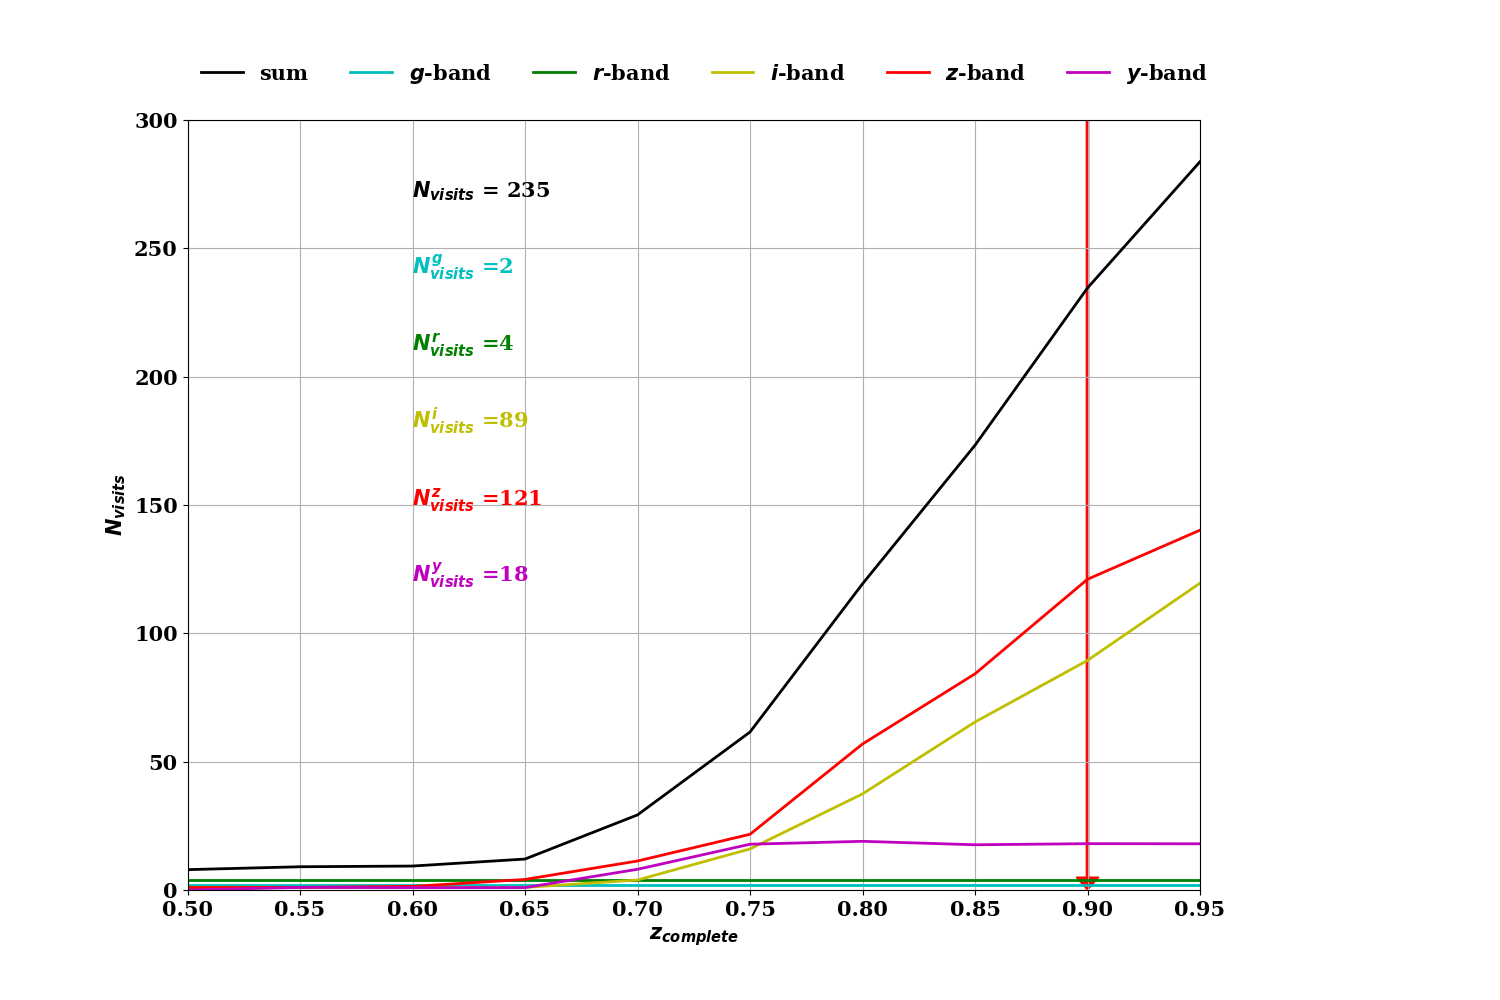
\includegraphics[width=0.95\textwidth]{nvisits_zlim.png}
 \caption{Number of visits as a function of the completeness redshift. 250 visits {\it with} the following filter allocation (\nvisitsall)=(2,2,98,130,18) are requested per observing night to reach \zcomp\seq0.9.}\label{fig:nvisits_zlim}
\end{center}
\end{figure}
We may then use \ref{eq:zliminvisits} and \ref{fig:nvisits_zlim} to estimate the redshift of completeness corresponding to the number of visits of \ref{tab:ddbudget}. The conclusions of the result (Tab. \ref{tab:zlim}) are (a) it is very difficult to reach completeness redshifts higher than 0.6-0.7 if all fields are observed for ten years ; (b) the only way to explore higher  redshift domains is to reduce the number of seasons of observation.

\begin{table}[!htbp]
  \caption{Redshift of completeness as a function of the DD budget and the cadence of observation for a configuration of 5 fields. The first/second number corresponds to 10/2 seasons of observation per field. The redshift of completeness are independent on the cadence since the total SNR per band, \snrb,are identical.}\label{tab:zlim}
  \begin{center}
    \begin{tabular}{c|c|c|c}
      \hline
      \hline
      \diagbox[innerwidth=3.cm,innerleftsep=-1.cm,height=3\line]{budget}{cadence} & 1 & 2 & 3\\
      \hline
      6\% &\multicolumn{3}{c}{0.62/0.74} \\
      10\% & \multicolumn{3}{c}{0.66/0.79} \\
      15\% & \multicolumn{3}{c}{0.68/0.83}\\
      \hline
    \end{tabular}
  \end{center}
\end{table}


\section{Rolling Deep Drilling scenarios: probing higher \zcomp~domains}
\label{sec:scenario}
\subsection{Season length and number of visits}
The season length of observation is a parameter involved in the estimation of the budget and the number of well-sampled \sne.  It depends on the position of the field (w.r.t. LSST position) but also on the number of visits per night. The season length may be estimated from a list of night during which a field is visible (i.e. with altitude 20$^o\leq$ alt$\leq$86.5$^o$ and airmass$\leq$1.5) for a duration corresponding to \nvisits.  The results is given on Fig. \ref{fig:seasonlength_nvisits}. The season lengths decrease from 275-200 to 150-100 days for \nvisits~increasing from 1 to 400.  Combining information of sec. \ref{sec:opti} and Fig. \ref{fig:seasonlength_nvisits} lead to the conclusion that low cadences are favored to reach higher \zcomp~values while maximizing the season length. This is due to the fact that the minimal \snrb~to reach \zcomp~is independent on the cadence. The corresponding requested number of visits increases with the cadence. This leads to a decrease of the season length.

\begin{figure}[htbp]
\begin{center}
  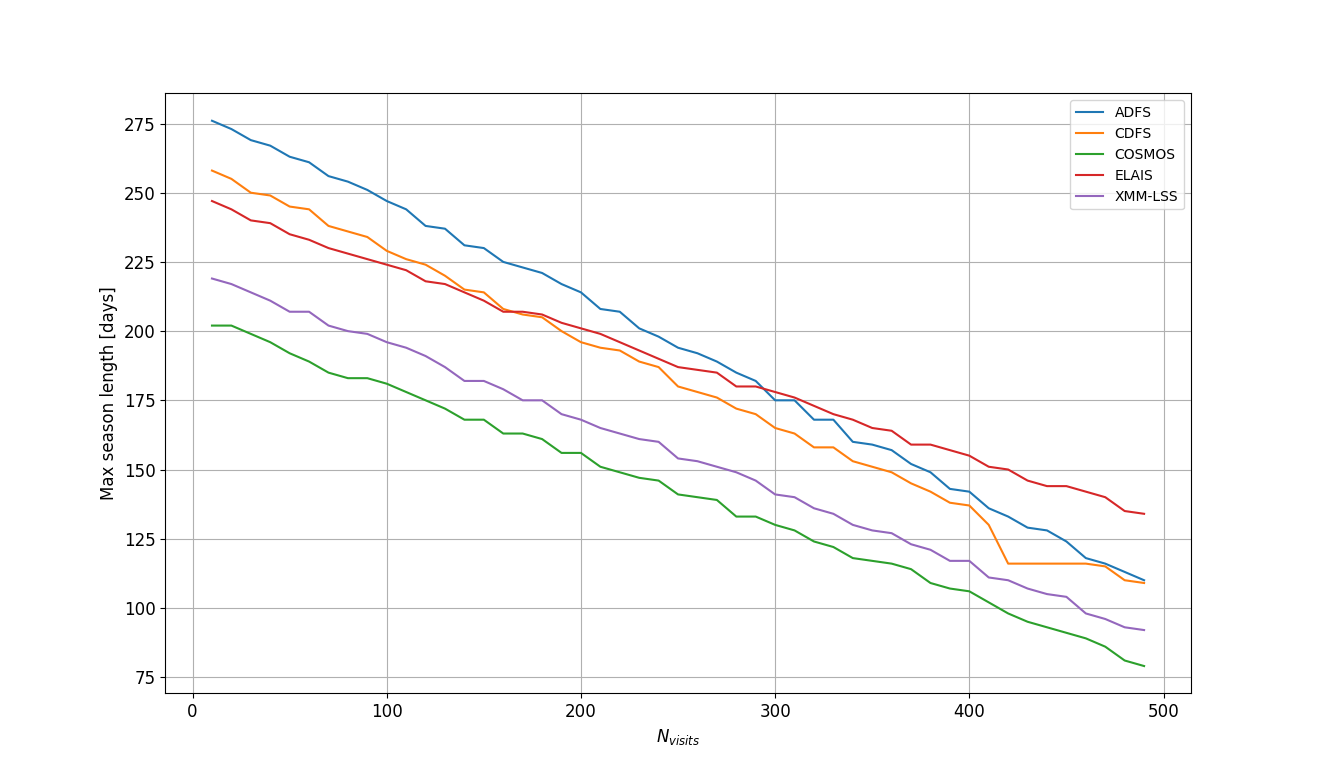
\includegraphics[width=0.95\textwidth]{seasonlength_nvisits.png}
 \caption{Maximal season length as a function of the number of visits.}\label{fig:seasonlength_nvisits}
\end{center}
\end{figure}

\subsection{Rolling Deep Drilling strategies}
A Deep Drilling program may be defined by seven parameters: the number of fields to observe, the number of season of observation (per field), the season length (per field), the number of visits (and filter distribution) per observing night, the budget, the number of supernovae, and the redshift of completeness. A GUI (Fig. \ref{fig:budget_gui}) was designed from the results of sec. \ref{sec:opti} to design Deep Drilling scenarios. Once the field parametersconfiguration (fields to observe, number of seasons, season length) is set, one of the three parameters (\zcomp, budget, \nvisits) may be fixed to estimate the two others. 

\begin{figure}[htbp]
\begin{center}
  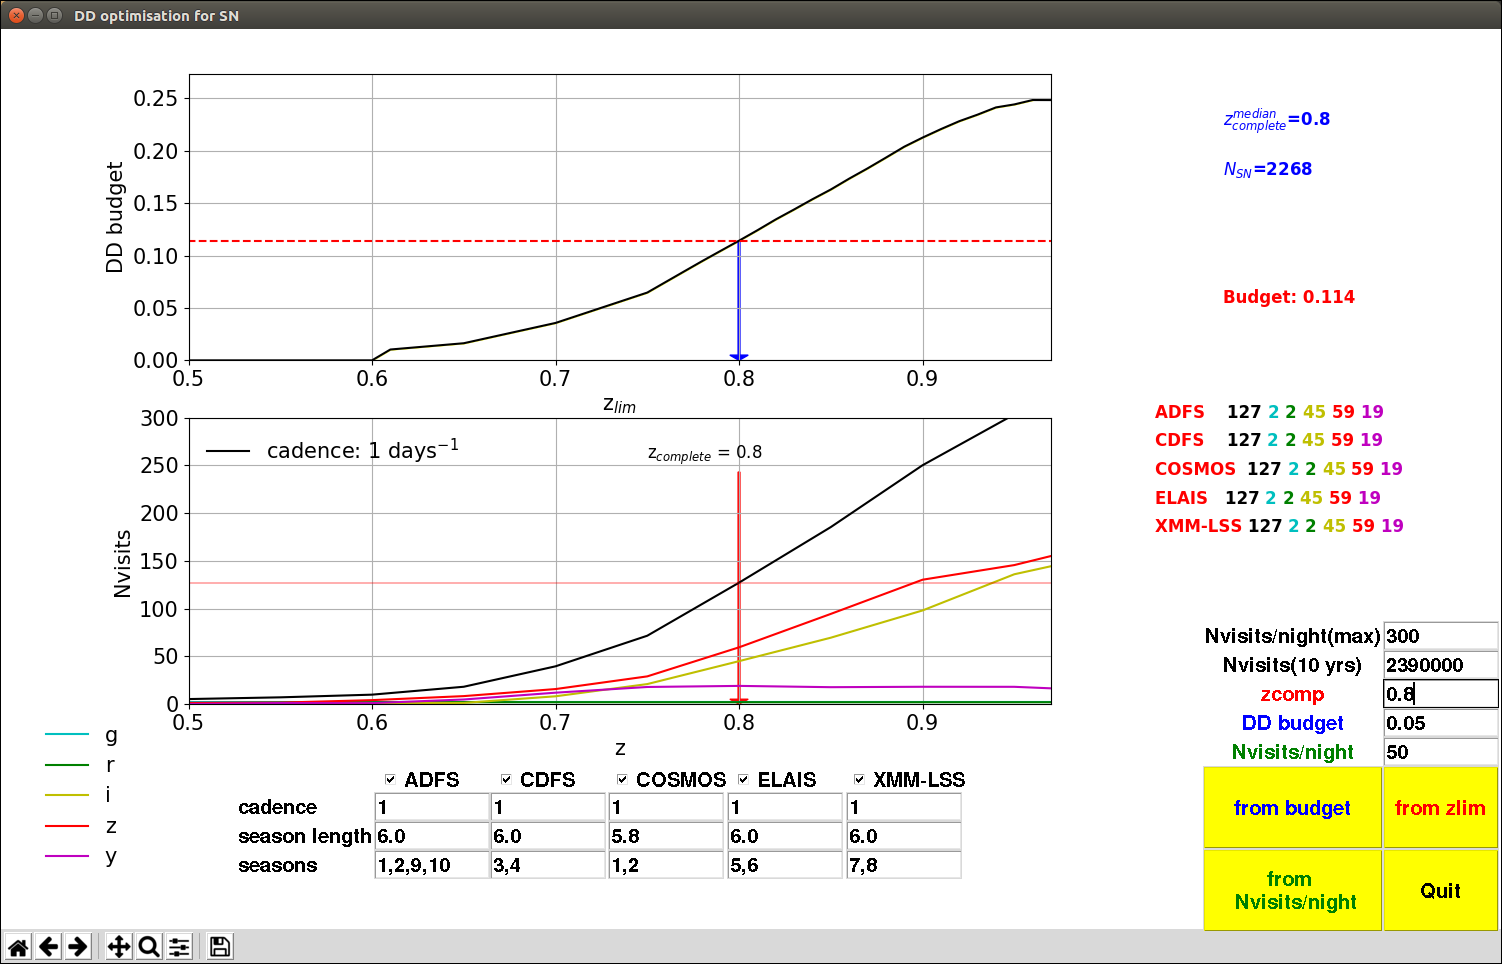
\includegraphics[width=0.95\textwidth]{budget_GUI.png}
 \caption{A GUI to define Deep Drilling programs. The field parameters (fields to observe, number of seasons, season length) are defined in the bottom table. The bottom plot displays the number of visits as a function of \zcomp. The budget as a function of \zcomp~is represented on the top plot. One of the three parameters (\zcomp, budget, \nvisits) may be fixed to estimate the two others. The expected total number of supernovae is also estimated. We have chosen \zcomp$\sim$0.8 as an illustraion.}\label{fig:budget_gui}
\end{center}
\end{figure}
Observing 5 fields for ten years up to \zcomp$\sim$ 0.9 would certainly give access to a large sample of well-measured \sne (around 11k) but also to an unrealistic scenario (budget: 87\%). This result confirm that the only way to reach higher \zcomp~while maintaining a reasonable budget is to reduce the number of seasons of observation. This is the purpose of the Rolling Deep Drilling (RDD) strategies presented in Tab. \ref{tab:rolling_scenarios}. We are presenting three scenarios, depending on the number of fields and for \zcomp~0.8,0.84,0.9. The budget ranges from 11\per~ to 15\per~and the number of supernovae between 1800 to 2500.

\begin{table}[!htbp]
  \caption{Set of scenarios to reach higher \zcomp.}\label{tab:rolling_scenarios}
  \begin{center}
    \begin{tabular}{c|c|c|c|c|c|c|c}
      \hline
      \hline
      Scenario & \zcomp & \nsncomp & budget & \nvisits & fields & seasons & season length\\
                       &                 &                     &               & \bg/\br/\bi/\bz/\by &        & & [month] \\
      \hline
      \multirow{5}{*}{\ddfscen{a}} & \multirow{5}{*}{0.8} & \multirow{5}{*}{2270} & \multirow{5}{*}{11.4\per} & & COSMOS & 1,2 & 5.8 \\
         &       &          &                  &          & CDFS         & 3,4 & 6.0 \\
         &       &          &                  &      127               & ELAIS        & 7,8 & 6.0 \\
         &       &          &                  &    2/2/45/58/19                  &XMM-LSS  & 9,10 & 6.0 \\
         &       &          &                  &                     &ADFS          & 1,2,5,6 & 6.0 \\
      \hline
      \multirow{5}{*}{\ddfscen{b}} & \multirow{5}{*}{0.84} & \multirow{5}{*}{2500} & \multirow{5}{*}{15.0\per} & & COSMOS & 1,2 & 5.4\\
         &       &          &                  &          & CDFS         & 3,4 & 6.0 \\
         &       &          &                  &      169               & ELAIS        & 7,8 & 6.0 \\
         &       &          &                  &    2/2/63/85/18                  &XMM-LSS  & 9,10 & 5.8\\
         &       &          &                  &                     &ADFS          & 1,2,5,6 & 6.0 \\
      \hline
      \multirow{3}{*}{\ddfscen{c}} & \multirow{3}{*}{0.9} & \multirow{3}{*}{1860} & \multirow{3}{*}{14.3\per} & & COSMOS & 1,2 & 4.7 \\
         &       &          &                  &     250     & CDFS         & 3,4 & 6.0 \\
         &       &          &                  &    2/2/98/130/18                 &ADFS          & 1,2,5,6 & 6.0 \\
      \hline
      \end{tabular}
  \end{center}
\end{table}



\subsection{Budget and \by-visits}

% ----------------------------------------------------------------------

\section{Type Ia supernovae as probe for assessing observing strategy}
\label{sec:snprobes}
Type Ia supernovae are transient astronomical events resulting from a powerful and luminous explosion of a white dwarf. They are identified by their brightness evolution, with a luminosity peak about 15 days after explosion, and a slow decrease lasting up to few months. It is expected that all type Ia supernovae observed in the DD fields in LSST will be identified from spectral features. Accurate supernova parameters will be estimated from well-measured light curves characterized by a sampling of few days and high Signal-to-Noise Ratio per band (\snrb). These two quality criteria are determined at the first order by two key parameters of observing strategies: the cadence of observation, and the number of visits per band.
\par
Rest-frame wavelengths of type Ia supernovae range from $\sim$380 nm (blue cut-off) to $\sim$800 nm (red cut-off). Since the flux fraction per band (observer frame) varies with the redshift, these two limits have an impact on the possible list of bands with minimal flux useable to observe supernovae (Tab. \ref{tab:zfilters}): only three bands (\bi\bz\by) are useable in the redshift range 0.64-0.98 and only two (\bz\by) for redshifts higher than $\sim$1. 

\begin{table}[!htbp]
  \caption{Available bands with minimal flux vs redshift.}\label{tab:zfilters}
  \begin{center}
    \begin{tabular}{c|c}
      \hline
      \hline
      Redshift range & available bands \\
      \hline
      0.01-0.1 & \bg\br\bi\\
      0.1-0.3 & \bg\br\bi\bz \\
      0.3-0.64 & \br\bi\bz\by \\
      0.64-0.98 & \bi\bz\by \\
      $\geq$ 0.98 & \bz\by \\
      \hline
      \end{tabular}
  \end{center}
\end{table}

Type Ia supernovae may be described by five parameters (\salt~model): stretch\strech, color \col, time of maximum luminosity \daymax, normalization of the SED \xnorm, and the redshift \z.  They are measured from light curve fits to estimate the Hubble diagram distance modulus:
\begin{equation}
  \mu =m_B^*- M_B+\alpha \times x_1 -\beta \times c \label{eq:mu}
\end{equation}
where $m_B^*$ corresponds to the observed peak magnitude in rest-frame B-band and $\alpha$($\simeq$ 0.14),$\beta$($\simeq$ 3.1) and $M_B$ are nuisance parameters. The distance modulus error \sigmu~is dominated by the error on the color \sigc: measuring $\mu$ at the precent level  requires to have \sigc$\lesssim$0.04.

Since \sigc~varies with the redshift  (Fig. \ref{fig:sigc_z}, top), the requirement \sigc$\lesssim$0.04 leads to a redshift limit value (0.61 in \ref{fig:sigc_z}, top) defining the limit of the completeness of the survey (\zlim) if \sigc~is estimated using faint type Ia supernovae with (\strech,\col)=(-2.0,0.2). One may also observe (\ref{fig:sigc_z}, bottom) that \sigc~also depends (as expected) on \snrb. This means that the condition \sigc$\lesssim$0.04 requires \snrb$\geq$\snrbmin, where \snrbmin~is a minimal signal-to-noise ratio for each of the bands available in the redshift range considered (Tab. \ref{tab:zfilters}).

\begin{figure}[htbp]
\begin{center}
  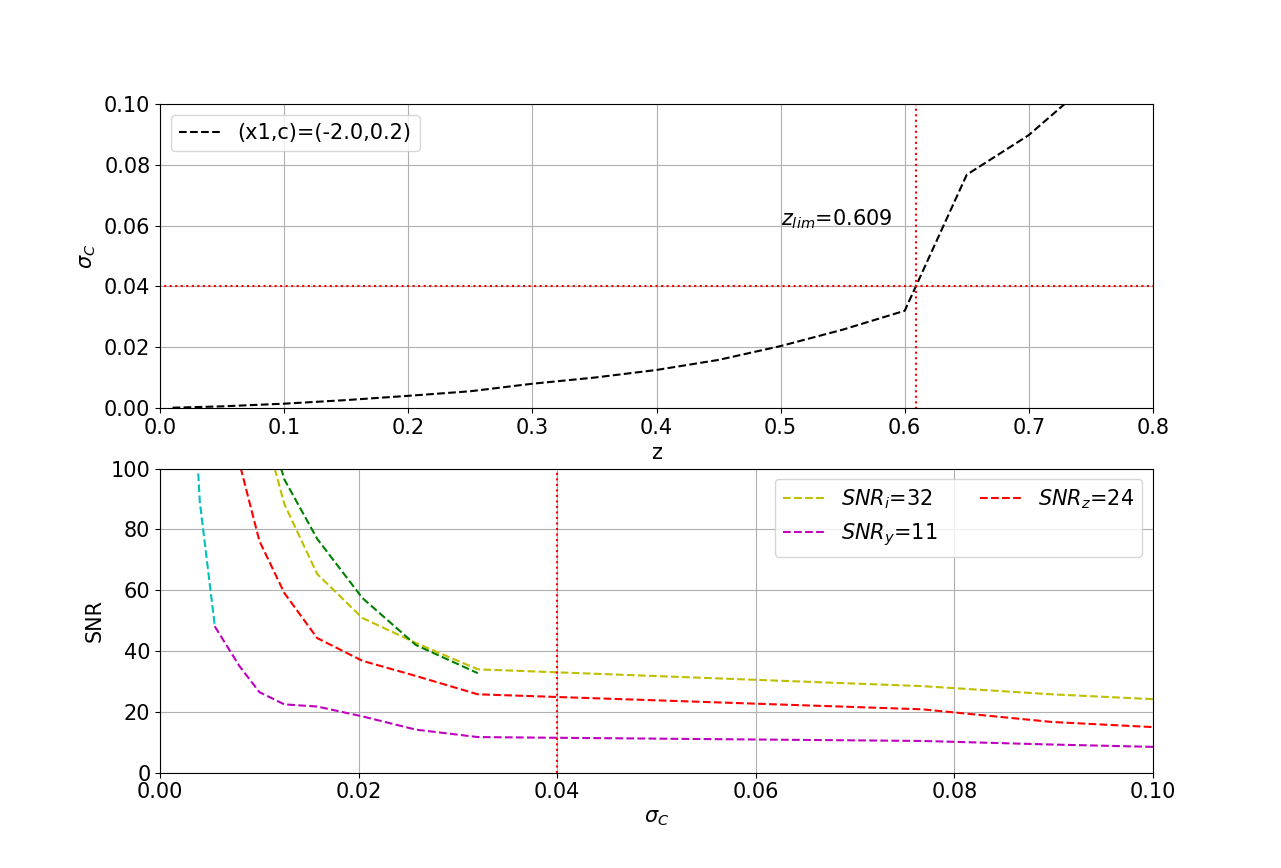
\includegraphics[width=0.9\textwidth]{sigmaC_z.png}
 \caption{Color error \sigc~as a function of redshift (top) and signal-to-noise ratio per band \snrb~as a function of \sigc~(bottom) for a faint type Ia supernova.}\label{fig:sigc_z}
\end{center}
\end{figure}



\section{LSST Deep Drilling program design constraints}
\label{sec:designb}

Up to approximately 10\% of LSST observing time will be dedicated to other programs, including intensive observation of a set of Deep Drilling Fields. 



\section{Analysis of recent simulations}

\begin{center} 
\begin{sidewaystable}[htbp] 
\resizebox{\textwidth}{!}{% 
\begin{tabular}{c|c|c|c|c|c|c|c|c|c} 
 Observing & DD frac(\%) & Field & cadence & Nvisits & m5 & Nnights & season length & total area & effective area \\ 
 Strategy &  &  & min/med/max & g/r/i/z/y & g/r/i/z/y & & [days] & [deg2] & [deg2] \\ 
\hline 
& & ADFS1 & 2/4/39 & 10/20/20/26/20 & 25.9/25.8/25.3/24.7/23.9 & 5/10/14 & 27/131/143 & 18 & 13 \\ 
& & ADFS2 & 2/4/39 & 10/20/20/26/20 & 25.9/25.8/25.4/24.7/23.9 & 5/10/14 & 27/131/143 & 18 & 14 \\ 
baseline\_v1.5\_10yrs& 4.6& CDFS & 2/10/58 & 10/20/20/26/20 & 25.7/25.7/25.2/24.6/23.7 & 5/16/27 & 39/200/229 & 18 & 14 \\ 
& & COSMOS & 1/4/38 & 10/20/20/26/20 & 25.7/25.6/25.2/24.7/23.8 & 5/16/26 & 27/164/185 & 17 & 15 \\ 
& & ELAIS & 2/4/38 & 10/20/20/26/20 & 25.8/25.7/25.2/24.8/23.8 & 5/17/26 & 13/150/170 & 18 & 15 \\ 
& & XMM-LSS & 2/5/37 & 10/20/20/26/20 & 25.7/25.6/25.2/24.7/23.7 & 5/16/26 & 29/152/171 & 18 & 15 \\ 
\hline 
& & ADFS1 & 2/2/35 & 2/4/8/25/4 & 24.8/24.8/24.8/24.8/23.1 & 5/43/86 & 14/147/158 & 18 & 17 \\ 
& & ADFS2 & 2/2/38 & 2/4/8/25/4 & 24.8/24.8/24.8/24.8/23.1 & 5/46/91 & 18/146/159 & 19 & 15 \\ 
descddf\_v1.5\_10yrs& 4.6& CDFS & 2/3/58 & 2/4/8/25/4 & 24.6/24.6/24.6/24.6/22.8 & 5/56/134 & 33/228/240 & 18 & 17 \\ 
& & COSMOS & 1/2/41 & 2/4/8/25/4 & 24.5/24.6/24.5/24.5/22.8 & 5/77/159 & 76/178/184 & 18 & 17 \\ 
& & ELAIS & 2/2/40 & 2/4/8/25/4 & 24.7/24.7/24.6/24.6/22.9 & 5/42/100 & 22/165/177 & 19 & 17 \\ 
& & XMM-LSS & 2/2/39 & 2/4/8/25/4 & 24.6/24.6/24.6/24.5/22.9 & 5/42/102 & 40/171/180 & 18 & 16 \\ 
\hline 
& & ADFS1 & 1/2/34 & 1/1/3/5/4 & 23.9/23.7/24.1/23.9/23.0 & 5/38/100 & 29/164/177 & 18 & 17 \\ 
& & ADFS2 & 1/2/37 & 1/1/3/5/4 & 23.9/23.7/24.1/23.9/23.0 & 5/42/100 & 29/165/177 & 19 & 16 \\ 
agnddf\_v1.5\_10yrs& 3.4& CDFS & 1/2/62 & 1/1/3/5/4 & 23.7/23.6/24.0/23.8/22.9 & 5/56/127 & 48/235/248 & 18 & 17 \\ 
& & COSMOS & 1/2/46 & 1/1/3/5/4 & 23.5/23.4/23.8/23.6/22.8 & 5/60/122 & 59/189/205 & 18 & 17 \\ 
& & ELAIS & 1/2/46 & 1/1/3/5/4 & 23.8/23.7/24.1/23.9/23.1 & 5/42/108 & 41/171/192 & 19 & 17 \\ 
& & XMM-LSS & 1/2/41 & 1/1/3/5/4 & 23.6/23.5/23.9/23.8/22.9 & 5/47/113 & 48/177/191 & 18 & 17 \\ 
\hline 
& & ADFS1 & 1/2/44 & 1/1/2/2/2 & 24.5/24.0/24.0/23.4/22.7 & 5/59/140 & 21/161/173 & 18 & 17 \\ 
& & ADFS2 & 1/2/33 & 1/1/2/2/2 & 24.5/24.1/24.0/23.4/22.7 & 5/66/140 & 22/161/173 & 19 & 16 \\ 
daily\_ddf\_v1.5\_10yrs& 5.5& CDFS & 1/2/30 & 1/1/2/2/2 & 24.2/23.8/23.8/23.2/22.5 & 5/77/202 & 38/236/246 & 18 & 17 \\ 
& & COSMOS & 1/2/42 & 1/1/2/2/2 & 24.0/23.7/23.7/23.0/22.3 & 5/81/167 & 45/188/203 & 18 & 17 \\ 
& & ELAIS & 1/2/37 & 1/1/2/2/2 & 24.3/23.9/23.8/23.2/22.6 & 5/57/143 & 52/171/182 & 19 & 17 \\ 
& & XMM-LSS & 1/2/40 & 1/1/2/2/2 & 24.1/23.8/23.7/23.1/22.4 & 5/65/149 & 38/178/188 & 19 & 17 \\ 
\end{tabular}} 
\end{sidewaystable} 
\end{center}
\begin{center} 
\resizebox{\textwidth}{!}{% 
\begin{tabular}{c|c|c|c|c|c|c|c|c|c} 
 Observing & DD budget(\%) & Field & cadence & Nvisits & Nnights & season length & area \\ 
 Strategy &  &  & min/med/max & g/r/i/z/y & & [days] & [deg2] \\ 
\hline 
& & ADFS1 & 2/4/34 & 10/20/20/26/20 & 5/11/13 & 11/121/148 & 15 \\ 
& & ADFS2 & 2/4/34 & 10/20/20/26/20 & 5/11/13 & 10/123/148 & 15 \\ 
ddf\_dither0.00\_v1.7\_10yrs& 4.6& CDFS & 3/6/15 & 10/20/20/26/20 & 10/21/26 & 62/204/228 & 9 \\ 
& & COSMOS & 2/2/10 & 10/20/20/26/20 & 18/22/24 & 142/165/177 & 10 \\ 
& & ELAIS & 2/3/17 & 10/20/20/26/20 & 5/22/24 & 68/153/168 & 8 \\ 
& & XMM-LSS & 2/3/13 & 10/20/20/26/20 & 7/22/25 & 58/159/172 & 9 \\ 
\hline 
& & ADFS1 & 2/4/32 & 10/20/20/26/20 & 5/11/15 & 28/116/149 & 15 \\ 
& & ADFS2 & 2/4/44 & 10/20/20/26/20 & 5/11/15 & 26/116/149 & 15 \\ 
ddf\_dither0.05\_v1.7\_10yrs& 4.6& CDFS & 2/6/27 & 10/20/20/26/20 & 5/21/25 & 52/218/228 & 9 \\ 
& & COSMOS & 2/2/30 & 10/20/20/26/20 & 5/22/24 & 78/168/177 & 10 \\ 
& & ELAIS & 2/3/35 & 10/20/20/26/20 & 5/22/24 & 49/153/168 & 9 \\ 
& & XMM-LSS & 2/3/29 & 10/20/20/26/20 & 5/23/24 & 54/161/169 & 10 \\ 
\hline 
& & ADFS1 & 1/4/29 & 10/20/20/26/20 & 5/11/13 & 8/120/145 & 15 \\ 
& & ADFS2 & 2/4/39 & 10/20/20/26/20 & 5/11/13 & 11/120/145 & 15 \\ 
ddf\_dither0.10\_v1.7\_10yrs& 4.6& CDFS & 2/6/45 & 10/20/20/26/20 & 5/21/25 & 56/220/228 & 10 \\ 
& & COSMOS & 2/2/29 & 10/20/20/26/20 & 5/21/24 & 46/165/177 & 10 \\ 
& & ELAIS & 2/3/39 & 10/20/20/26/20 & 5/22/24 & 50/150/168 & 11 \\ 
& & XMM-LSS & 2/3/37 & 10/20/20/26/20 & 5/22/25 & 32/165/172 & 10 \\ 
\hline 
& & ADFS1 & 2/4/32 & 10/20/20/26/20 & 5/10/13 & 28/118/148 & 15 \\ 
& & ADFS2 & 2/4/32 & 10/20/20/26/20 & 5/11/13 & 27/118/148 & 15 \\ 
ddf\_dither0.30\_v1.7\_10yrs& 4.6& CDFS & 2/6/50 & 10/20/20/26/20 & 5/20/25 & 49/201/230 & 13 \\ 
& & COSMOS & 2/3/47 & 10/20/20/26/20 & 5/21/24 & 33/167/177 & 12 \\ 
& & ELAIS & 2/3/38 & 10/20/20/26/20 & 5/21/25 & 28/146/168 & 13 \\ 
& & XMM-LSS & 2/3/44 & 10/20/20/26/20 & 5/21/25 & 37/146/174 & 13 \\ 
\hline 
& & ADFS1 & 2/4/39 & 10/20/20/26/20 & 5/11/13 & 28/123/157 & 15 \\ 
& & ADFS2 & 2/4/31 & 10/20/20/26/20 & 5/11/13 & 29/137/157 & 15 \\ 
ddf\_dither0.70\_v1.7\_10yrs& 4.6& CDFS & 2/9/63 & 10/20/20/26/20 & 5/14/25 & 29/201/228 & 18 \\ 
& & COSMOS & 2/4/42 & 10/20/20/26/20 & 5/17/24 & 26/163/177 & 17 \\ 
& & ELAIS & 2/4/42 & 10/20/20/26/20 & 5/17/25 & 28/146/168 & 18 \\ 
& & XMM-LSS & 2/4/40 & 10/20/20/26/20 & 5/15/24 & 34/146/169 & 18 \\ 
\hline 
& & ADFS1 & 2/4/31 & 10/20/20/26/20 & 5/10/13 & 24/113/147 & 15 \\ 
& & ADFS2 & 2/4/32 & 10/20/20/26/20 & 5/10/13 & 24/118/147 & 15 \\ 
ddf\_dither1.00\_v1.7\_10yrs& 4.6& CDFS & 2/14/55 & 10/20/20/26/20 & 5/11/25 & 49/198/230 & 23 \\ 
& & COSMOS & 2/5/47 & 10/20/20/26/20 & 5/13/24 & 32/153/177 & 23 \\ 
& & ELAIS & 2/5/44 & 10/20/20/26/20 & 5/12/25 & 13/143/177 & 23 \\ 
& & XMM-LSS & 2/5/47 & 10/20/20/26/20 & 5/12/25 & 39/143/172 & 23 \\ 
\hline 
& & ADFS1 & 2/4/39 & 10/20/20/26/20 & 5/10/13 & 27/121/145 & 15 \\ 
& & ADFS2 & 2/4/31 & 10/20/20/26/20 & 5/10/13 & 27/121/145 & 15 \\ 
ddf\_dither1.50\_v1.7\_10yrs& 4.6& CDFS & 2/16/59 & 10/20/20/26/20 & 5/10/25 & 28/196/230 & 31 \\ 
& & COSMOS & 2/8/49 & 10/20/20/26/20 & 5/10/24 & 30/145/174 & 32 \\ 
& & ELAIS & 2/6/42 & 10/20/20/26/20 & 5/10/24 & 27/135/168 & 32 \\ 
& & XMM-LSS & 2/6/45 & 10/20/20/26/20 & 5/10/25 & 26/139/176 & 32 \\ 
\hline 
& & ADFS1 & 2/4/39 & 10/20/20/26/20 & 5/10/13 & 23/112/149 & 15 \\ 
& & ADFS2 & 2/4/33 & 10/20/20/26/20 & 5/10/13 & 23/111/149 & 15 \\ 
ddf\_dither2.00\_v1.7\_10yrs& 4.6& CDFS & 2/19/58 & 10/20/20/26/20 & 5/9/20 & 29/193/229 & 41 \\ 
& & COSMOS & 2/12/46 & 10/20/20/26/20 & 5/8/20 & 29/137/173 & 42 \\ 
& & ELAIS & 2/9/52 & 10/20/20/26/20 & 5/9/22 & 21/118/168 & 42 \\ 
& & XMM-LSS & 2/9/50 & 10/20/20/26/20 & 5/9/22 & 22/133/174 & 41 \\ 
\end{tabular}} 
\end{sidewaystable} 
\end{center}
\begin{center} 
\begin{sidewaystable}[htbp] 
\resizebox{\textwidth}{!}{% 
\begin{tabular}{c|c|c|c|c|c|c|c|c|c} 
 Observing & DD frac(\%) & Field & cadence & Nvisits & m5 & Nnights & season length & total area & effective area \\ 
 Strategy &  &  & min/med/max & g/r/i/z/y & g/r/i/z/y & & [days] & [deg2] & [deg2] \\ 
\hline 
& & ADFS1 & 2/4/34 & 10/20/20/26/20 & 25.8/25.8/25.3/24.7/23.9 & 5/11/13 & 11/121/148 & 15 & 12 \\ 
& & ADFS2 & 2/4/34 & 10/20/20/26/20 & 25.9/25.8/25.3/24.8/23.9 & 5/11/13 & 10/123/148 & 15 & 12 \\ 
ddf\_dither0.00\_v1.7\_10yrs& 4.6& CDFS & 3/6/15 & 10/20/20/26/20 & 25.6/25.6/25.2/24.6/23.6 & 10/21/26 & 62/204/228 & 9 & 9 \\ 
& & COSMOS & 2/2/10 & 10/20/20/26/20 & 25.6/25.6/25.2/24.7/23.8 & 18/22/24 & 142/165/177 & 10 & 10 \\ 
& & ELAIS & 2/3/17 & 10/20/20/26/20 & 25.7/25.7/25.2/24.8/23.8 & 5/22/24 & 68/153/168 & 8 & 8 \\ 
& & XMM-LSS & 2/3/13 & 10/20/20/26/20 & 25.6/25.6/25.1/24.7/23.7 & 7/22/25 & 58/159/172 & 9 & 9 \\ 
\hline 
& & ADFS1 & 2/4/32 & 10/20/20/26/20 & 25.8/25.8/25.3/24.6/23.9 & 5/11/15 & 28/116/149 & 15 & 13 \\ 
& & ADFS2 & 2/4/44 & 10/20/20/26/20 & 25.8/25.8/25.3/24.7/23.9 & 5/11/15 & 26/116/149 & 15 & 12 \\ 
ddf\_dither0.05\_v1.7\_10yrs& 4.6& CDFS & 2/6/27 & 10/20/20/26/20 & 25.6/25.6/25.2/24.6/23.7 & 5/21/25 & 52/218/228 & 9 & 9 \\ 
& & COSMOS & 2/2/30 & 10/20/20/26/20 & 25.6/25.6/25.2/24.7/23.8 & 5/22/24 & 78/168/177 & 10 & 10 \\ 
& & ELAIS & 2/3/35 & 10/20/20/26/20 & 25.7/25.6/25.2/24.8/23.8 & 5/22/24 & 49/153/168 & 9 & 9 \\ 
& & XMM-LSS & 2/3/29 & 10/20/20/26/20 & 25.6/25.6/25.2/24.7/23.7 & 5/23/24 & 54/161/169 & 10 & 10 \\ 
\hline 
& & ADFS1 & 1/4/29 & 10/20/20/26/20 & 25.8/25.8/25.3/24.7/23.9 & 5/11/13 & 8/120/145 & 15 & 11 \\ 
& & ADFS2 & 2/4/39 & 10/20/20/26/20 & 25.9/25.8/25.3/24.7/23.9 & 5/11/13 & 11/120/145 & 15 & 12 \\ 
ddf\_dither0.10\_v1.7\_10yrs& 4.6& CDFS & 2/6/45 & 10/20/20/26/20 & 25.6/25.6/25.1/24.6/23.6 & 5/21/25 & 56/220/228 & 10 & 10 \\ 
& & COSMOS & 2/2/29 & 10/20/20/26/20 & 25.6/25.6/25.1/24.7/23.8 & 5/21/24 & 46/165/177 & 10 & 10 \\ 
& & ELAIS & 2/3/39 & 10/20/20/26/20 & 25.7/25.6/25.2/24.8/23.8 & 5/22/24 & 50/150/168 & 11 & 10 \\ 
& & XMM-LSS & 2/3/37 & 10/20/20/26/20 & 25.6/25.5/25.1/24.7/23.7 & 5/22/25 & 32/165/172 & 10 & 10 \\ 
\hline 
& & ADFS1 & 2/4/32 & 10/20/20/26/20 & 25.8/25.8/25.4/24.7/23.9 & 5/10/13 & 28/118/148 & 15 & 11 \\ 
& & ADFS2 & 2/4/32 & 10/20/20/26/20 & 25.9/25.8/25.3/24.7/23.9 & 5/11/13 & 27/118/148 & 15 & 12 \\ 
ddf\_dither0.30\_v1.7\_10yrs& 4.6& CDFS & 2/6/50 & 10/20/20/26/20 & 25.6/25.6/25.1/24.7/23.7 & 5/20/25 & 49/201/230 & 13 & 12 \\ 
& & COSMOS & 2/3/47 & 10/20/20/26/20 & 25.6/25.6/25.1/24.7/23.7 & 5/21/24 & 33/167/177 & 12 & 11 \\ 
& & ELAIS & 2/3/38 & 10/20/20/26/20 & 25.7/25.7/25.2/24.7/23.8 & 5/21/25 & 28/146/168 & 13 & 12 \\ 
& & XMM-LSS & 2/3/44 & 10/20/20/26/20 & 25.6/25.5/25.1/24.7/23.7 & 5/21/25 & 37/146/174 & 13 & 11 \\ 
\hline 
& & ADFS1 & 2/4/39 & 10/20/20/26/20 & 25.8/25.8/25.3/24.5/23.9 & 5/11/13 & 28/123/157 & 15 & 12 \\ 
& & ADFS2 & 2/4/31 & 10/20/20/26/20 & 25.8/25.8/25.3/24.7/23.9 & 5/11/13 & 29/137/157 & 15 & 13 \\ 
ddf\_dither0.70\_v1.7\_10yrs& 4.6& CDFS & 2/9/63 & 10/20/20/26/20 & 25.6/25.6/25.2/24.6/23.7 & 5/14/25 & 29/201/228 & 18 & 14 \\ 
& & COSMOS & 2/4/42 & 10/20/20/26/20 & 25.6/25.6/25.1/24.7/23.7 & 5/17/24 & 26/163/177 & 17 & 15 \\ 
& & ELAIS & 2/4/42 & 10/20/20/26/20 & 25.7/25.7/25.2/24.8/23.8 & 5/17/25 & 28/146/168 & 18 & 15 \\ 
& & XMM-LSS & 2/4/40 & 10/20/20/26/20 & 25.6/25.5/25.1/24.7/23.7 & 5/15/24 & 34/146/169 & 18 & 15 \\ 
\end{tabular}} 
\end{sidewaystable} 
\end{center}
\begin{center} 
\begin{sidewaystable}[htbp] 
\resizebox{\textwidth}{!}{% 
\begin{tabular}{c|c|c|c|c|c|c|c|c|c} 
 Observing & DD frac(\%) & Field & cadence & Nvisits & m5 & Nnights & season length & total area & effective area \\ 
 Strategy &  &  & min/med/max & g/r/i/z/y & g/r/i/z/y & & [days] & [deg2] & [deg2] \\ 
\hline 
& & ADFS1 & 2/4/31 & 10/20/20/26/20 & 25.8/25.8/25.4/24.7/23.9 & 5/10/13 & 24/113/147 & 15 & 12 \\ 
& & ADFS2 & 2/4/32 & 10/20/20/26/20 & 25.8/25.7/25.3/24.7/23.9 & 5/10/13 & 24/118/147 & 15 & 12 \\ 
ddf\_dither1.00\_v1.7\_10yrs& 4.6& CDFS & 2/14/55 & 10/20/20/26/20 & 25.6/25.6/25.1/24.6/23.7 & 5/11/25 & 49/198/230 & 23 & 18 \\ 
& & COSMOS & 2/5/47 & 10/20/20/26/20 & 25.6/25.6/25.2/24.7/23.8 & 5/13/24 & 32/153/177 & 23 & 17 \\ 
& & ELAIS & 2/5/44 & 10/20/20/26/20 & 25.7/25.6/25.2/24.7/23.8 & 5/12/25 & 13/143/177 & 23 & 18 \\ 
& & XMM-LSS & 2/5/47 & 10/20/20/26/20 & 25.6/25.6/25.1/24.7/23.7 & 5/12/25 & 39/143/172 & 23 & 19 \\ 
\hline 
& & ADFS1 & 2/4/39 & 10/20/20/26/20 & 25.8/25.8/25.3/24.7/23.9 & 5/10/13 & 27/121/145 & 15 & 13 \\ 
& & ADFS2 & 2/4/31 & 10/20/20/26/20 & 25.8/25.8/25.3/24.8/23.9 & 5/10/13 & 27/121/145 & 15 & 12 \\ 
ddf\_dither1.50\_v1.7\_10yrs& 4.6& CDFS & 2/16/59 & 10/20/20/26/20 & 25.6/25.6/25.1/24.6/23.7 & 5/10/25 & 28/196/230 & 31 & 22 \\ 
& & COSMOS & 2/8/49 & 10/20/20/26/20 & 25.6/25.6/25.1/24.7/23.7 & 5/10/24 & 30/145/174 & 32 & 23 \\ 
& & ELAIS & 2/6/42 & 10/20/20/26/20 & 25.7/25.7/25.2/24.8/23.8 & 5/10/24 & 27/135/168 & 32 & 22 \\ 
& & XMM-LSS & 2/6/45 & 10/20/20/26/20 & 25.6/25.5/25.1/24.7/23.7 & 5/10/25 & 26/139/176 & 32 & 22 \\ 
\hline 
& & ADFS1 & 2/4/39 & 10/20/20/26/20 & 25.8/25.8/25.3/24.7/23.9 & 5/10/13 & 23/112/149 & 15 & 13 \\ 
& & ADFS2 & 2/4/33 & 10/20/20/26/20 & 25.8/25.7/25.3/24.7/23.9 & 5/10/13 & 23/111/149 & 15 & 12 \\ 
ddf\_dither2.00\_v1.7\_10yrs& 4.6& CDFS & 2/19/58 & 10/20/20/26/20 & 25.6/25.6/25.1/24.6/23.6 & 5/9/20 & 29/193/229 & 41 & 25 \\ 
& & COSMOS & 2/12/46 & 10/20/20/26/20 & 25.6/25.6/25.2/24.7/23.7 & 5/8/20 & 29/137/173 & 42 & 26 \\ 
& & ELAIS & 2/9/52 & 10/20/20/26/20 & 25.7/25.7/25.2/24.7/23.8 & 5/9/22 & 21/118/168 & 42 & 27 \\ 
& & XMM-LSS & 2/9/50 & 10/20/20/26/20 & 25.6/25.6/25.1/24.7/23.7 & 5/9/22 & 22/133/174 & 41 & 26 \\ 
\end{tabular}} 
\end{sidewaystable} 
\end{center}


% ----------------------------------------------------------------------

%\section{Lessons from recent simulations}
%\label{sec:simu}


% ----------------------------------------------------------------------

\section{Optimization of the LSST Deep Drilling  program}
\label{sec:optimization}
\subsection{Optimization method}


\subsection{Results}

% ----------------------------------------------------------------------


\section{Proposal for new DD-minisurvey scenario}
\label{sec:proposal}

% ----------------------------------------------------------------------

\section{Discussion}
\label{sec:discussion}



% ----------------------------------------------------------------------

\section{Conclusion}
\label{sec:conclusion}



% ----------------------------------------------------------------------

\subsection*{Acknowledgments}

%%% Here is where you should add your specific acknowledgments, remembering that some standard thanks will be added via the \code{desc-tex/ack/*.tex} and \code{contributions.tex} files.

%This paper has undergone internal review in the LSST Dark Energy Science Collaboration. % REQUIRED if true

Author contributions are listed below. \\
Ph.~Gris: conceptualization,software,analysis,writing \\
N.~Regnault: conceptualization,writing \\
 % Standard papers only: author contribution statements. For examples, see http://blogs.nature.com/nautilus/2007/11/post_12.html

% This work used TBD kindly provided by Not-A-DESC Member and benefitted from comments by Another Non-DESC person.

% Standard papers only: A.B.C. acknowledges support from grant 1234 from ...

\input{desc-tex/ack/standard} % also available: key standard_short

% This work used some telescope which is operated/funded by some agency or consortium or foundation ...

% We acknowledge the use of An-External-Tool-like-NED-or-ADS.

%{\it Facilities:} \facility{LSST}

% Include both collaboration papers and external citations:
\bibliography{main,lsstdesc}

\end{document}

% ======================================================================
